%%%%%%%%%%%%%%%%%%%%%%%%%%%%%%%%%%%%%%%%%%%%%%%%%%%%%%%%%%%%%%%%%%%%%%%%%%%%%%%%
%2345678901234567890123456789012345678901234567890123456789012345678901234567890
%        1         2         3         4         5         6         7         8

\documentclass[letterpaper, 10 pt, conference]{ieeeconf}  % Comment this line out
                                                          % if you need a4paper
%\documentclass[a4paper, 10pt, conference]{ieeeconf}      % Use this line for a4
                                                          % paper

\IEEEoverridecommandlockouts                              % This command is only
                                                          % needed if you want to
                                                          % use the \thanks command
\overrideIEEEmargins
% See the \addtolength command later in the file to balance the column lengths
% on the last page of the document



% The following packages can be found on http:\\www.ctan.org
%\usepackage{graphics} % for pdf, bitmapped graphics files
%\usepackage{epsfig} % for postscript graphics files
%\usepackage{mathptmx} % assumes new font selection scheme installed
%\usepackage{times} % assumes new font selection scheme installed
%\usepackage{amsmath} % assumes amsmath package installed
%\usepackage{amssymb}  % assumes amsmath package installed
\usepackage{graphicx}

\title{\LARGE \bf
Rossmann Store Sales
}

%\author{ \parbox{3 in}{\centering Huibert Kwakernaak*
%         \thanks{*Use the $\backslash$thanks command to put information here}\\
%         Faculty of Electrical Engineering, Mathematics and Computer Science\\
%         University of Twente\\
%         7500 AE Enschede, The Netherlands\\
%         {\tt\small h.kwakernaak@autsubmit.com}}
%         \hspace*{ 0.5 in}
%         \parbox{3 in}{ \centering Pradeep Misra**
%         \thanks{**The footnote marks may be inserted manually}\\
%        Department of Electrical Engineering \\
%         Wright State University\\
%         Dayton, OH 45435, USA\\
%         {\tt\small pmisra@cs.wright.edu}}
%}

\author{Bharadiya Pavan(MT2018023) and Devarakonda Deepak(MT2018031)% <-this % stops a space
}


\begin{document}


\maketitle
\thispagestyle{empty}
\pagestyle{empty}


%%%%%%%%%%%%%%%%%%%%%%%%%%%%%%%%%%%%%%%%%%%%%%%%%%%%%%%%%%%%%%%%%%%%%%%%%%%%%%%%
\begin{abstract}

Sales forecasting is a common topic in business.The task is to forecast the "Sales" for 1,115 stores located across Germany
for a given day. Store sales are influenced by many factors. Our project aims to create a robust prediction model.
We tried different models like linear regression,decision tree,random forest,XGBoost to predict sales for a given day. XGBoost turned out to be the best model. Then We tried stacking of random forest and XGBoost and tried to blend them with original features as well. Final selected model was stacking giving 0.05788 RMSPE on public leaderboard and 0.05602 on private leaderboard. We also observed that "Customers" column was the most important feature for sales prediction.   

\end{abstract}


%%%%%%%%%%%%%%%%%%%%%%%%%%%%%%%%%%%%%%%%%%%%%%%%%%%%%%%%%%%%%%%%%%%%%%%%%%%%%%%%
\section{INTRODUCTION}

Rossmann operates over 3,000 drug stores in 7 European countries. Currently, Rossmann store managers are tasked with predicting their daily sales for up to six weeks in advance. Store sales are influenced by many factors, including promotions, competition, school and state holidays, seasonality, and locality. With thousands of individual managers predicting sales based on their unique circumstances, the accuracy of results can be quite varied. Competition is to predict sales for a given day for 1,115 stores located across Germany. Reliable sales forecasts enable store managers to create effective staff schedules that increase productivity and motivation. 

The given features are mostly store related and there is only one column which is related to customer which shows the total customer visiting the store. As the target is continuous, the problem could be a regression problem based on both categorical feature(e.g,  Store Type,Assortment,StateHoliday) and continuous feature(e.g, Days). Besides, some feature could be considered as categorical as well as continuous,  for example,  DayOfWeek could be considered as continuous by
[1,2,3,4,5,6,7], assuming there is a relationship for adjacent days or as categorical [Mon, Tue, Wed, Thu, Fri, Sat, Sun],assuming there is no relationship between them.

\section{DATASET}

\subsection{Data Collection}

This project was hosted on kaggle as InClass competition where data is provided which contains four files - train.csv, store.csv, test.csv and samplesubmission.csv. you can find the data at https://www.kaggle.com/c/iiitb-ml-project-rossmann-store-sales/data

\subsection{Description Of The Dataset}\bigskip

\textbf{train.csv} \bigskip

This is the main training dataset which contains data about the sales figures for a store on a particular date.

Data Fields:

\textbf{1. Store ​ :} a unique numerical store identifier (1 - 1,115)

\textbf{2. DayOfWeek ​ :} the day of week (1 - 7)

\textbf{3. Date ​ :} the date from 2013-01-01 to 2015-07-17

\textbf{4. Sales ​ :} the turnover of a store on the specified date

\textbf{5. Customers ​ :}the number of customers of a store

\textbf{6. Open ​ :}  (0 = Closed, 1 = Open)

\textbf{7. Promo ​ :} indicates promotion(0 = No, 1 = Yes)

\textbf{8. StateHoliday ​ :}shows type of state holiday

\textbf{9. SchoolHoliday ​ :} (0 = No, 1 = Yes)

\textbf{10. Id :} Unique id for all data

\textbf{No. of Records:​} 1,000,000\bigskip

\textbf{store.csv}\bigskip

This dataset contains supplementary information about each of the 1,115 stores and helps identify unique features which may (or may not) affect sales.

Data Fields:

\textbf{1. Store ​ :} a unique numerical store identifier (1 - 1,115)

\textbf{2. StoreType ​ :} 4 different types of stores (a, b, c, d)

\textbf{3. Assortment ​ :} describes the assortment of goods 

(a = Basic, b = Extra, c = Extended)

\textbf{4. CompetitionDistance ​ :} the distance (in metres) to the 

nearest competitor’s store

\textbf{5. CompetitionOpenSinceMonth ​ :} the month in which 

the competition opened

\textbf{6. CompetitionOpenSinceYear ​ :} the year in which the 

competition opened

\textbf{7. Promo2 ​ :} indicates if a store is participating in a 

continuing and consecutive promotion(0 = No, 1 = Yes)

\textbf{8. Promo2SinceWeek ​ :} the week of the year in which 

the store began participating in Promo2 ​ (from 1 - 50,

presumably, but some weeks are unrepresented in the data)

\textbf{9. Promo2SinceYear ​ :} the year in which the store began 

participating in ​ Promo2 (from 2009 - 2015)

\textbf{10. PromoInterval ​ :} describes the consecutive intervals 

in which ​ Promo2 is activated, giving the 

months the promotion is renewed (either “Jan,Apr,Jul,Oct”, 

“Feb,May,Aug,Nov” or “Mar,Jun,Sept,Dec”)

\textbf{No. of Records :} 1,115\bigskip



\textbf{test.csv}\bigskip

This dataset is to be used for testing and evaluating the model.
Data Fields: Same as train.csv, with the exclusion of Sales.

\textbf{No. of Records :} 1115



\section{Preprocessing The Data}
\subsubsection{\textbf{Open column}}

Removing all those entries where store is closed as sales is zero.
\bigskip
\subsubsection{\textbf{CompetitionDistance}}

Replacing NaN values with 0 since no record was there.
\bigskip
\subsubsection{\textbf{CompetitionSince[X]}}

Replacing all the NaN values with 0 for for CompetitionSinceYear and CompetitionSinceMonth
respectively.

\bigskip
\subsubsection{\textbf{Promo2Since[X]}}

Replacing all the NaN values with 0 for for Promo2SinceYear and Promo2SinceWeek respectively.

\bigskip
\subsubsection{\textbf{StateHoliday}}
Converting all 0(integer) to "0"(String) because data in the StateHoliday is a mix of numerical and string values. Hence, for the sake of consistency,all values were converted to string.

\bigskip
\subsubsection{\textbf{Label Encoding}}

we performed label encoding on the categorical features present in our dataset, including StateHoliday in train.csv and test.csv and  StoreType  and Assortment  in store.csv.

\bigskip
\section{Exploratory Data Analysis}

The  following  subsections  are  trying  to  analyze  dataset and  figure  out  useful  features  that  can  be  used  to  forecast sales. At first, we will attempt to extract features from training dataset. Then, in order to get more useful features, the store information will be reviewed. At last,  we will try to get more information from what we have now based on store
information.

\subsection{Correlation Between Training data} 

\begin{figure}[h!]
  \centering
  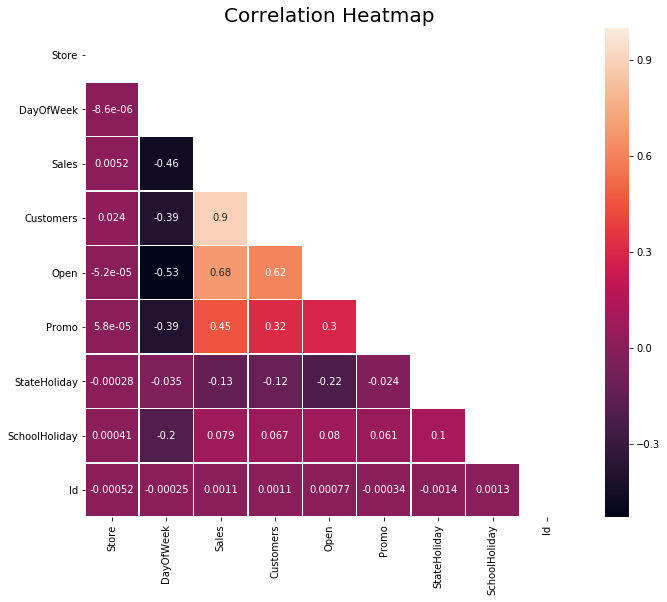
\includegraphics[width=20cm,height=7cm,keepaspectratio]{corr.png}
  \caption{correlation matrix}
\end{figure}


\subsubsection{\textbf{Store ID}}

It is customary to think the store ID as one feature because
sales may change from store to store. However, if we just use
the Store ID as one feature, we will find that the correlation coefficient between Store ID and Sales is only 0.0052.

\subsubsection{\textbf{Day of Week}}
It’s also easy to think that in different day of week, every
store will have different sales since people get used to shop
in different days. The day of week seems to have large effect
on sales as we can see that the correlation coefficient is -0.46.

\subsubsection{\textbf{Number of Customers}}
In the training dataset which represents the past information includes the numbers of customers. This is also present in test.csv and it is very highly correlated with sales. We can see that the correlation coefficient is 0.9.

\subsubsection{\textbf{Open}}
Open shows whether this store is open or not in a specified day. Because  the  sales  must  be  0  when  the  store  is
closed, we removed the data point with "Open = 0" and after
prediction, we would set the value of sales as 0 for the data
point with Open = 0 in testing data. We can see that the correlation coefficient is 0.68.

\subsubsection{\textbf{Promo}}
It indicates whether a store is running a promo on that day.
As  promotion  would  be  a  attracting  thing  for customer, it might have effect on the sales.So correlation coefficient is 0.45.

\subsection{Frequency Distribution}
\textbf{1) Frequency Of Sales}
\begin{figure}[h!]
    \centering
    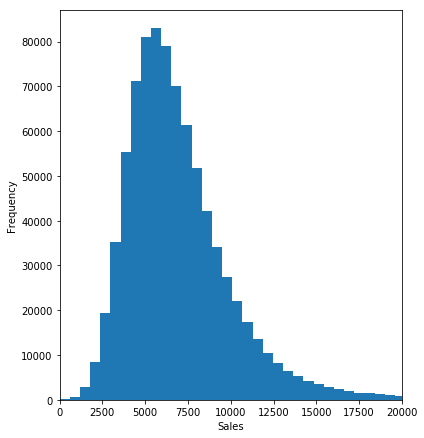
\includegraphics[width=6cm,height=6cm]{freq-sales.png}
    \caption{frequency of sales}
\end{figure}

By looking at the chart above, we can see that the Sales values forms a Poisson-like distribution, reaching its peak of frequency between 5,000 and 7,500. At the same time, it is uncommon for ​ Sales to fall below 2,500 (on open days) or go beyond 12,500.The average value for ​ Sales for open stores is 6,914.95.\bigskip


%\subsubsection{Frequency of customers}
\textbf{2)Frequency Of Customers}
\begin{figure}[h!]
    \centering
    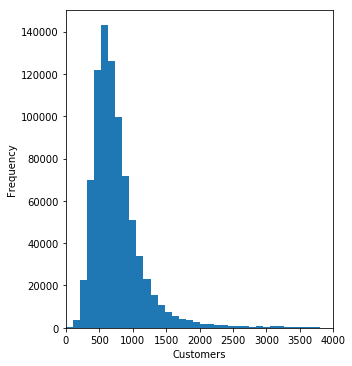
\includegraphics[width=6cm,height=5cm]{freq-cust.png}
    \caption{frequency of customers}
\end{figure}

Similarly, the distribution of Customers values follows a Poisson-like distribution, indicating that the number of customers commonly ranges between 500 and 1,000, while a value higher than 1,000 has relatively low frequency. The average value for ​ Customers for open stores is 762.56.

\subsection{Possible Outliers}
We can check the max,min and average values of sales which shows that minimum value = 527, maximum value = 38722, mean value is = 6914 and 75 percetile = 8209 which is very less than max sales.

Sales $>$  35,000 = 7

Sales $>$  30,000 = 48

Sales $>$ 25,000 = 308

This suggests that Sales values greater than 30,000 can be safely ignored to avoid overfitting as those records are extremely rare and only occur in a handful of stores but could affect the model’s predictions for the other stores.

\subsection{Trends For DayOfWeek}
\textbf{1) mean(Sales) v/s DayOfWeek}

\begin{figure}[h!]
    \centering
    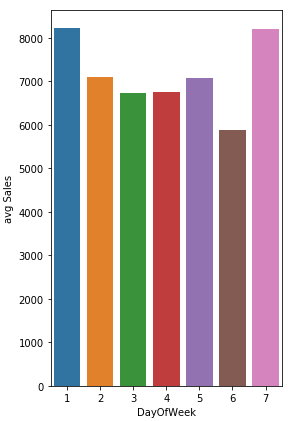
\includegraphics[width=7cm,height=6cm]{sales-DOW.png}
    \caption{sales for all Days of week}
\end{figure}

\textbf{2) Customers v/s DayOfWeek}

\begin{figure}[h!]
    \centering
    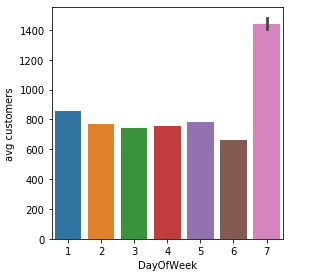
\includegraphics[width=7cm,height=8cm,keepaspectratio]{customers-DOW.png}
    \caption{mean(customers) for all days of week}
\end{figure}

From the above graphs we can see that, there are three peaks in the average sales and average no.
of customers in the week. The first two are on Mondays and Fridays, which is probably due to
these days being the start and end of the week. The highest peak, however, is on
Sundays, which is probably due to the fact that most other stores are closed. An interesting
observation here is that there is a larger difference between the average no. of customers and
average sales on Sundays as compared to other days of the week. While the average sales is
approximately the same on Sundays and Mondays, there is a drastic difference in the no. of
customers, which hints at a large number of window shoppers on Sundays.

\subsection{Monthly trends}
\bigskip
\textbf{1)Monthly mean(Sales)}

\begin{figure}[h!]
    \centering
    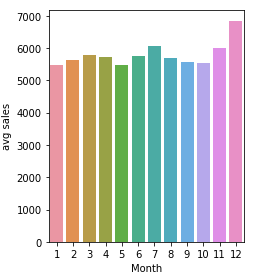
\includegraphics[width=7cm,height=9cm]{sales-months.png}
    \caption{mean(sales) for all months}
\end{figure}


\textbf{2)Monthly mean(Customers)}

\begin{figure}[h!]
    \centering
    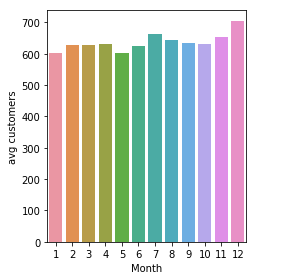
\includegraphics[width=15cm,height=6cm,keepaspectratio]{customers-months.png}
    \caption{mean(customers) for all months}
\end{figure}

When plotting the average sales and no. of customers by month, we see an annual trend similar
to most retail stores. There is an uptick in the months of June - July owing to summer
holidays and another bigger uptick in December, which is likely due to the holiday season.


\subsection{Average percentage change in sales annually}


\begin{figure}[h!]
    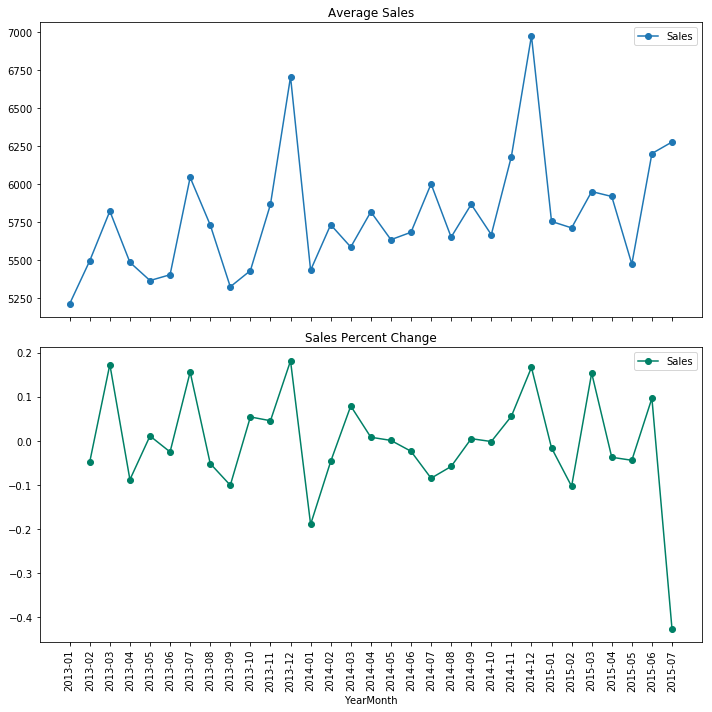
\includegraphics[width=0.5\textwidth]{download.png}
\end{figure}
%\begin{figure}[h!]
%    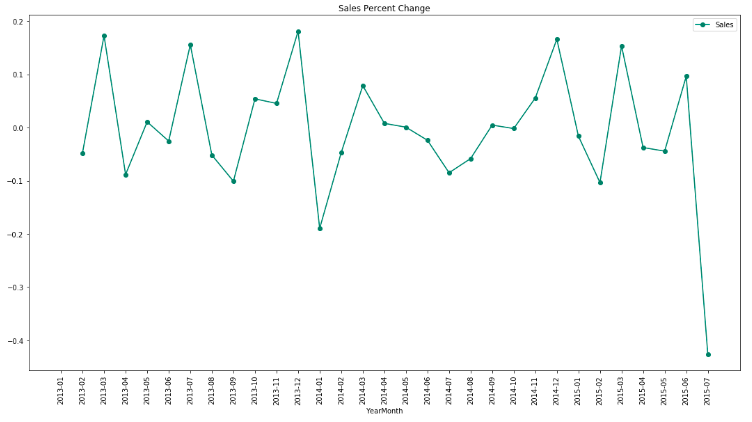
\includegraphics[width=8.5cm,height=10cm,keepaspectratio]{avgsales-pct1.png}
%    \caption{percentage change in sales annually}
%\end{figure}

The annual trends are further corroborated when plotting the average sales data per month for the entirety of the training dataset (January 2013 to July 2015). We see the same annual trends being followed in the 2.5 years, with increasing peak values every year hinting at improved store performance from 2013 to 2014 to 2015.

\subsection{Effect Of Promo}
\textbf{1) Effect Of Promo On Sales}

\begin{figure}[h!]
    \centering
    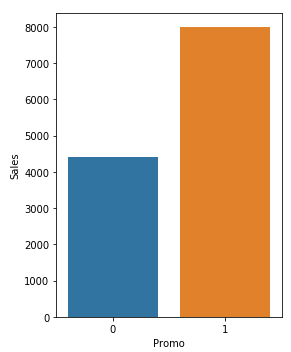
\includegraphics[width=6cm,height=5cm]{sales-promo.png}
    \caption{sales for promo}
\end{figure}

\bigskip
\bigskip

\textbf{2) Effect Of Promo On Customers}

\begin{figure}[h!]
    \centering
    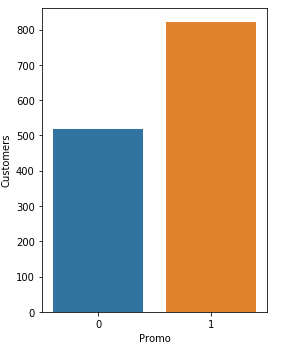
\includegraphics[width=6cm,height=5cm]{customers-promo.png}
    \caption{Customers for promo}
\end{figure}

The figure below shows the average customers and average sales (across all stores) on days
with and without promotions. The effect of having a promotion on sales and customers is
clearly evident, with the promotion having a strong positive effect on both.

\subsection{Effect Of StateHoliday}

\textbf{1)Total state holidays of different types}

\begin{figure}[h!]
    \centering
    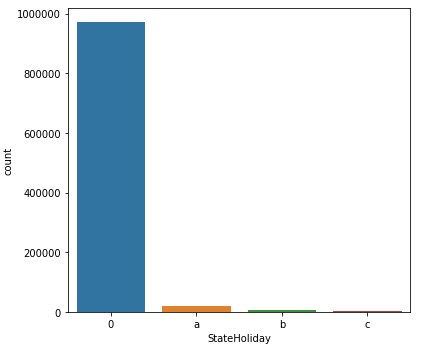
\includegraphics[width=8cm,height=5cm]{stateholiday.png}
    \caption{different types of state holidays}
\end{figure}

\textbf{2)Sales and Customers on state holiday}

\begin{figure}[h!]
    \centering
    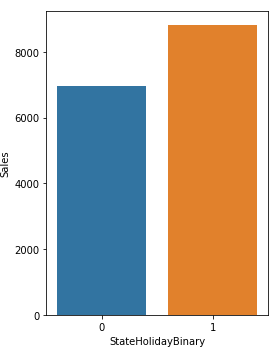
\includegraphics[width=6cm,height=6cm]{sales-SH.png}
    \caption{Sales of BinaryStateHoliday}
\end{figure}

\bigskip

\begin{figure}[h!]
    \centering
    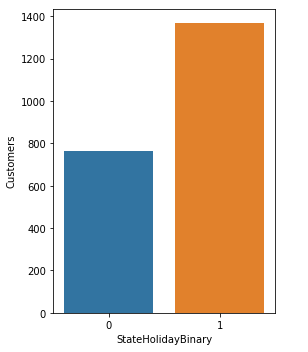
\includegraphics[width=6cm,height=6cm]{customers-SH.png}
    \caption{Customers of BinaryStateHoliday}
\end{figure}

from the first figure we can see that state holiday = 0 means no holiday which has most of the entries. 
Since most stores are closed on public holidays and closed stores can be ignored when
making predictions, the average sales figures and average number of customers on state
holidays is plotted, but only for open stores in the figure below. It is evident that when a store
is open on state holidays, it attracts more customers and accrues more sales.



\section{Feature Engineering}
Initially We merge train and Store csv files and do feature engineering on them as both files contains valuable information.

\subsubsection{\textbf{SalesPerCustomer}}

As the sales and customers are 

highly correlated, we can create new feature called Sales-

PerCustomer.

\subsubsection{\textbf{AvgSales}}

Group by the Store and calculate the mean 

value of sales for all the store and merge this new
data-

frame with store.csv using 'Store' as index and use as 

a new feature.

\subsubsection{\textbf{AvgCustomers}}

As customers are also very important 

we also group them
by the Store and calculate the mean 

value of customers for all store and merge this new 

dataframe with store.csv using 'Store' as index and use as 

a new feature.

\subsubsection{\textbf{AvgSalesCustomers}}

Do the same thing for AvgSales-

PerCustomer.

In the same way, instead of using mean we use meadian 

to calculate three more features called

\subsubsection{\textbf{MedSales}} Using median values of sales for all store
\subsubsection{\textbf{MedCustomers}} Using median values of customers for 

all store
\subsubsection{\textbf{MedSalesPerCustomers}} Using median values of sales 

per customer for all store

\subsubsection{\textbf{Year}} Using Date column
\subsubsection{\textbf{Month}} Using Date column
\subsubsection{\textbf{DayOfMonth}} Using Date column
\subsubsection{\textbf{DayOfYear}} Using Date column
\subsubsection{\textbf{WeekOfYear}} Using Date column


\subsubsection{\textbf{CompetitionOpen}}

We converted CompetitionOpen-

SinceYear and CompetitionOpenSinceMonth to all 

Months by doing CompetitionOpenSinceYear*12 - 

CompetitionOpenSincemonth  and stored it in Competi-

tionOpen

\subsubsection{\textbf{WeeksPromoOpen}}

We converted Promo2SinceYear 

and Promo2SinceWeek to all weeks and by doing 12 * 

(Year - Promo2SinceYear) + (Date.weekofyear -
Promo

2SinceWeek) / 4.0 and stored in WeeksPromoOpen


\subsubsection{\textbf{IsPromoMonth}}

This shows the current month is 

promo month or not. It is calculated using PromoInterval


column. 

Along with these 15 features some other features which 

we used directly are
\subsubsection{\textbf{Store}} Denotes store from 1 - 1115
\subsubsection{\textbf{Customers}} Customers for that store
\subsubsection{\textbf{CompetitionDistance}} Distance to competitors
\subsubsection{\textbf{Promo}} Indicates promo is there or not
\subsubsection{\textbf{Promo2}} indicates if a store is participating in a 

continuing and consecutive promotion

These are the all features we are using to train our model.
\subsection{Effect Of CompetitionDistance on AvgSales and AvgCustomers}

\begin{figure}[h!]
    \centering
    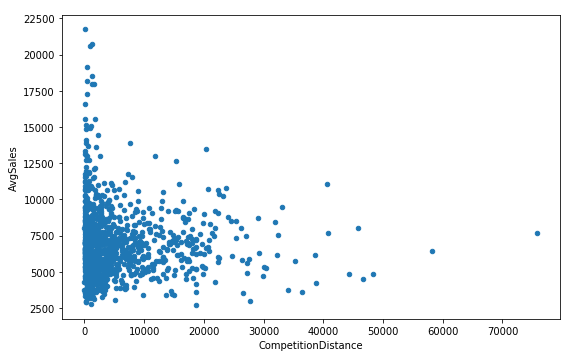
\includegraphics[width=8cm,height=6cm]{sales-CD.png}
    \caption{distance vs. AvgSales}
\end{figure}

\bigskip


\begin{figure}
    \centering
    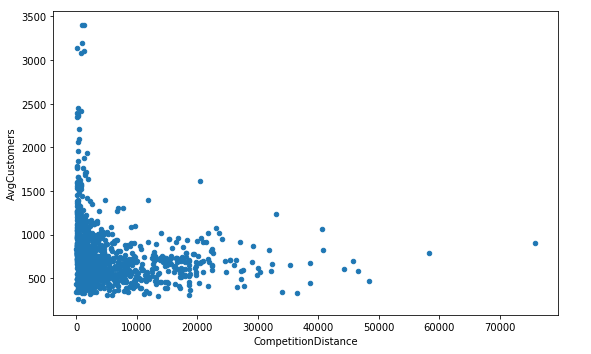
\includegraphics[width=8cm,height=6cm]{avgcust-CD.png}
    \caption{distance vs. AvgCustomers}
\end{figure}

From above graphs we can see that higher average sales  and average customer figures are achieved when
CompetitionDistance equals 0, or in other words, there is no nearby competition.

\subsection{Variation of AvgSales and AvgCustomers with StoreType}

\begin{figure}[h!]
    \centering
    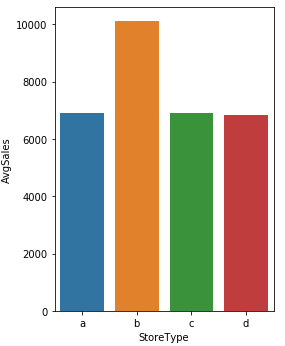
\includegraphics[width=5cm,height=5cm]{avgsales-St.png}
    \caption{StoreType vs. AvgSales}
\bigskip
\bigskip
    \centering
    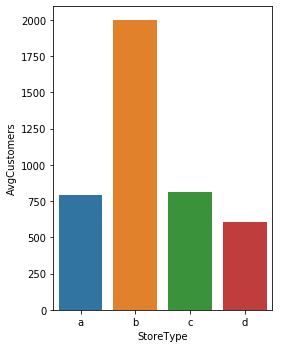
\includegraphics[width=5cm,height=5cm]{avgcust-ST.png}
    \caption{StoreType vs. AvgCustomers}
\end{figure}

A plot of the average sales and average customers of each store type shows that there is a strong correlation between the store type and average sales.

\section{Model Selection}
We used different models such as linear regression,decision tree regressor,random forest regressor and XGBoost regressor. We also tried blending and stacking of models. The RMSPE for the following models on our machine on validation data and on public leaderboard are as follows:
\bigskip

\textbf{Linear Regression:}

We got RMSPE = 0.085

public leaderboard score = 0.087
\bigskip

\textbf{DecisionTreeRegressor:}

We got RMSPE = 0.069

public leaderboard score = 0.072
\bigskip

\textbf{RandomForestRegressor:}

We got RMSPE = 0.058

public leaderboard score = 0.065

\bigskip
\textbf{XGBoostRegressor:}

We got RMSPE = 0.054

public leaderboard score = 0.062

\bigskip
\textbf{Blending random forest and xgboost with features and using xgboost:}

We got RMSPE = 0.055

public leaderboard score = 0.59

\bigskip
\textbf{Stacking random forest and xgboost and applying xgboost:}

We got RMSPE = 0.054

public leaderboard score = 0.057

\bigskip

For stacking and blending, we tried different splitting of the data. We tried training first random forest and XGBoost with 50\%,60\%,70\% of the data and then trained XGBoost again on the test\_size with previous model's output to predict for the test.csv. We got best results by training on 60\% data initially and training XGBoost again on remaining 40\% of the data.  

\bigskip

We tuned parameters for Random Forest and XgBoost using GridSearchCV.
The parameters used for random forest are as follows.

\bigskip

randomForest=RandomForestRegressor(n\_estimators=100, max\_depth=100, min\_samples\_leaf=1, min\_samples\_split=20, bootstrap=True, verbose=1, n\_jobs=-1)

\bigskip

The parameters used for XGBoost are as follows:

\bigskip

xgb.XGBRegressor(n\_jobs=-1,n\_estimators=4000,learning

\_rate=0.1,max\_depth=2,min\_child\_weight=2,subsample=

0.8,colsample\_bytree=0.8,tree\_method='exact',

reg\_alpha=0.05,silent=0,random\_state=1023)

\newpage
\section{Feature Importance Plots}
\subsection{Random Forest}
\begin{figure}[h!]
    \centering
    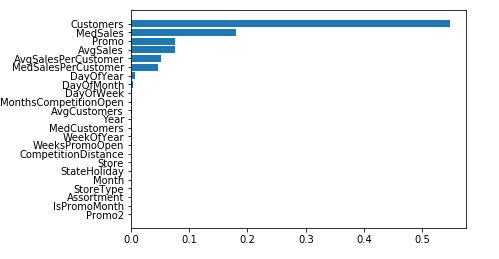
\includegraphics[width=0.5\textwidth]{importance-RF.png}
    \caption{random forest feature importance}
\end{figure}
The most important features for random forest are Customers,MedSales,AvgSales,AvgSalesPerCustomer,
DayOfYear,DayOfMonth.
\subsection{XGBoost}
\begin{figure}[h!]
    \centering
    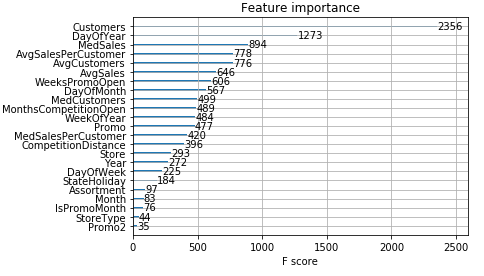
\includegraphics[width=0.5\textwidth]{importance-XGB.png}
    \caption{XGBoost feature importance}
\end{figure}
The most important features for XGBoost are Customers,DayOfYear,MedSales,AvgSalesPerCustomer,
AvgCustomers,AvgSales,WeeksPromoMonth,DayOfMonth.

\subsection{Stacking of Random Forest and XGBoost}
\begin{figure}[h!]
    \centering
    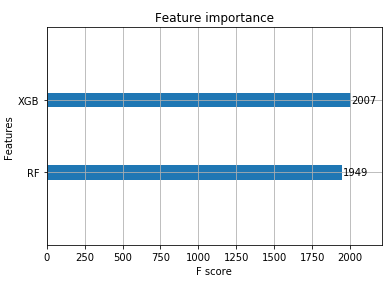
\includegraphics[width=8cm,height = 4.7cm]{importance-stack.png}
    \caption{Stacking feature importance}
\end{figure}
It is giving more importance to the XGBoost as shown in above figure.
\section{CONCLUSIONS}

We selected stacking and blending models as our two final models because they performed well on public leaderboad. Stacking model performed better on private leaderboard giving RMSPE of 0.05602 and using that we finished on third position. We observed that when the store is closed, value for Sales is 0. So for the test.csv,we predicted 0 when store was closed. The most important feature is Customer as it is highly correlated with Sales. Other important features were MedSales,DayOfYear,DayOfmonth,AvgSalesPerCustomers,
WeeksPromoOpen. On the private leaderboard, we observed
that our best score was RMSPE=0.05488 which was using only XGBoost but we didn't selected that as our final model to be evaluated as other models were performing better than only XGBoost.

\addtolength{\textheight}{-12cm}   % This command serves to balance the column lengths
                                  % on the last page of the document manually. It shortens
                                  % the textheight of the last page by a suitable amount.
                                  % This command does not take effect until the next page
                                  % so it should come on the page before the last. Make
                                  % sure that you do not shorten the textheight too much.

%%%%%%%%%%%%%%%%%%%%%%%%%%%%%%%%%%%%%%%%%%%%%%%%%%%%%%%%%%%%%%%%%%%%%%%%%%%%%%%%



%%%%%%%%%%%%%%%%%%%%%%%%%%%%%%%%%%%%%%%%%%%%%%%%%%%%%%%%%%%%%%%%%%%%%%%%%%%%%%%%



%%%%%%%%%%%%%%%%%%%%%%%%%%%%%%%%%%%%%%%%%%%%%%%%%%%%%%%%%%%%%%%%%%%%%%%%%%%%%%%%





\begin{thebibliography}{99}

\bibitem{c1} https://www.kaggle.com/c/rossmann-store-sales.
\bibitem{c2} https://www.analyticsvidhya.com/blog/2018/06/comprehensive-guide-for-ensemble-models/
\bibitem{c3} https://machinelearningmastery.com/xgboost-python-mini-course/
\bibitem{c4} https://seaborn.pydata.org/generated/seaborn.countplot.html?highlight

=countplots
\bibitem{c5} https://towardsdatascience.com/hyperparameter-tuning-the-random-forest-in-python-using-scikit-learn-28d2aa77dd74.


\end{thebibliography}




\end{document}
